\section{Experimental System}\label{sec:experimental_system}

Two separate experimental systems were used when testing and gathering results for localization and motion planning. The first of these is the physical robot, HARLIE, which will be described in further detail in \autoref{subsec:harlie_setup}. The second experimental system is a simulation environment which will be described in detail in \autoref{subsec:simulation_setup}.

\subsection{HARLIE}\label{subsec:harlie_setup}

\begin{figure}
\centering
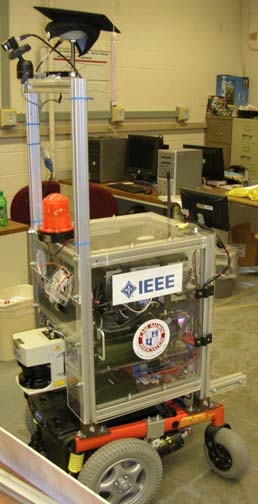
\includegraphics[height=0.5\textheight]{images/harlie}
\caption{HARLIE, the robot used for experimental testing \label{fig:harlie}}
\end{figure}

The physical robot used for these experiments was HARLIE (see \autoref{fig:harlie}). HARLIE is a fully autonomous robot built on top of a wheelchair base donated by the Invacare Corportation. The robot is powered via a pair of car batteries in series, providing a nominal twenty-four volts to the system. The wheelchair base has two electric motors powering the two drive wheels; with one motor per wheel, HARLIE is able to vary the velocity of each drive wheel independently. Because of this independent velocity control, HARLIE can move forwards and backwards, both straight and in arcs, as well as spin in place. This drive setup is known as ``differential drive'' and is one of the most common drive setups used in mobile robotics \autocite{Lav06}.

On top of this differential drive base, HARLIE is equipped with numerous sensors and computing systems. HARLIE is equipped with three sensors that are used for indoor localization: quadrature encoders, a MEMS gyroscope and a LIDAR. The quadrature encoders on HARLIE are used to measure the speed of each of HARLIE's drive wheels; these speeds are then integrated over time to get an estimate of the total distance moved by each wheel. HARLIE also has encoders attached to the two drive shafts, though these are used in the velocity control loops and not for localization. The encoders used on HARLIE (see \autoref{fig:grayhill_encoder}) are high-resolution optical encoders, providing over 1000 encoder ticks per wheel revolution (or approximately 58 $\mu$m per tick), which allows for precise measurement of the wheel's speed and direction. The encoders are not directly connected to the wheel's axle - they are connected via a pair of sprockets and a rubber, toothed belt (see \autoref{fig:wheel_encoder_setup}).

\begin{figure}
\centering
\subfloat[Grayhill 61K Optical Encoder]{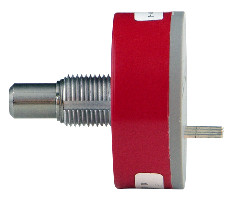
\includegraphics[width=0.5\textwidth]{images/grayhill_encoder}\label{fig:grayhill_encoder}}
\hfill
\subfloat[Wheel Encoder Setup]{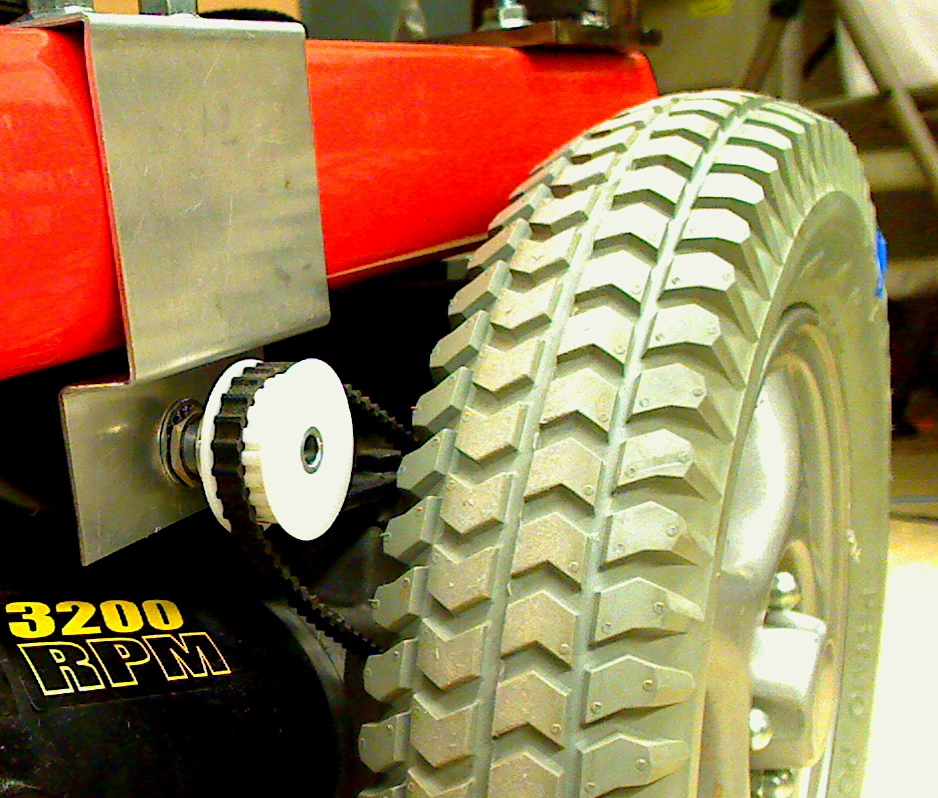
\includegraphics[width=0.5\textwidth]{images/wheel_encoder_setup}\label{fig:wheel_encoder_setup}}
\caption{Encoder \& Encoder setup}
\label{fig:encoder_and_setup}
\end{figure}

The second sensor on HARLIE used for indoor localization is an Analog Devices MEMS gyroscope (see \autoref{fig:yaw_rate_sensor}). This is a single-axis gyro used to measure the yaw rate (or angular velocity about the origin of rotation) of the robot. The sensor can measure a yaw rate of up to $\pm2.6$ radians per second and includes both a temperature sensor output as well as reference voltage output \autocite{ADXRS150Datasheet}. These latter outputs are important for correcting the sensor bias automatically - without bias correction, the yaw rate reading from the gyro will drift and give erroneous readings. With bias correction (see \autoref{subsec:relative_localization} for how this correction is done), the gyro is a very accurate estimator of HARLIE's yaw rate, even when there is wheel slippage that can cause errors in an yaw rate estimate derived from differencing the velocities of each drive wheel as reported by the encoders.

\begin{figure}
\centering
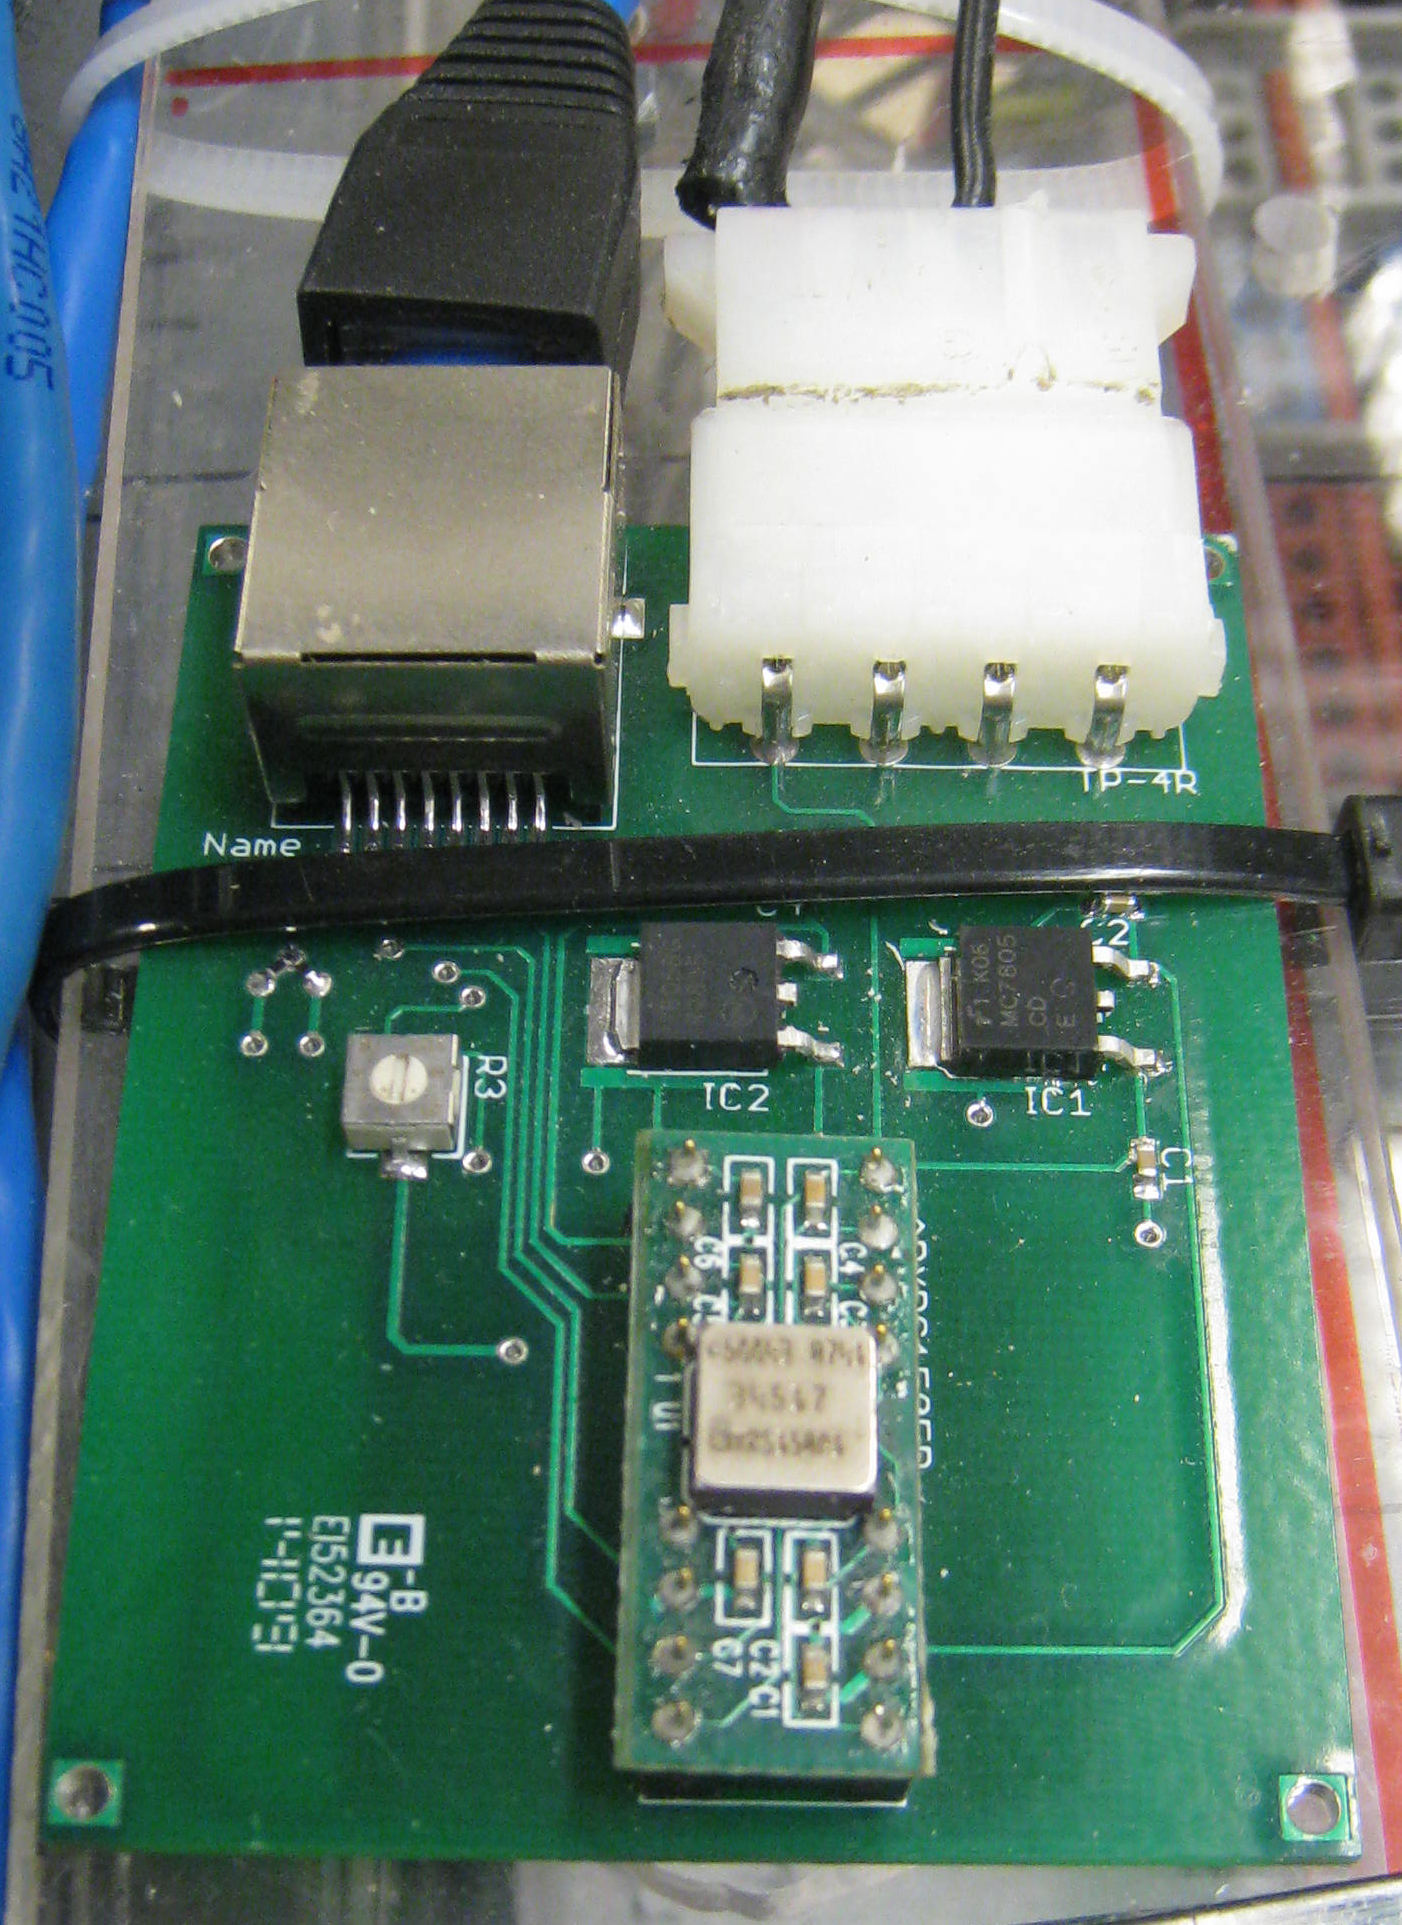
\includegraphics[width=0.5\textwidth]{images/yaw_rate_sensor}
\caption{Analog Devices ADXRS150 Gyro as mounted on HARLIE \label{fig:yaw_rate_sensor}}
\end{figure}

The third sensor on HARLIE used for indoor localization is the SICK LIDAR (see \autoref{fig:sick_lms291}). This LIDAR (LIght Detection And Ranging) unit uses a beam of infrared light (905nm wavelength) to scan in 1\degree{} increments a 180\degree{} arc in front of the sensor, returning a complete 180\degree{} scan at a rate of 75Hz (see \autoref{fig:sample_sick_scan}). The LMS291 can detect objects out to a range of 80 meters with an accuracy of $\pm1$ centimeter \autocite{SICKLMS291Datasheet}. With this long range and excellent accuracy, the SICK is able to provide enough information to localize HARLIE precisely in an indoor environment (see \autoref{subsec:absolute_localization} for details). 

\begin{figure}
\centering
\subfloat[SICK LMS291]{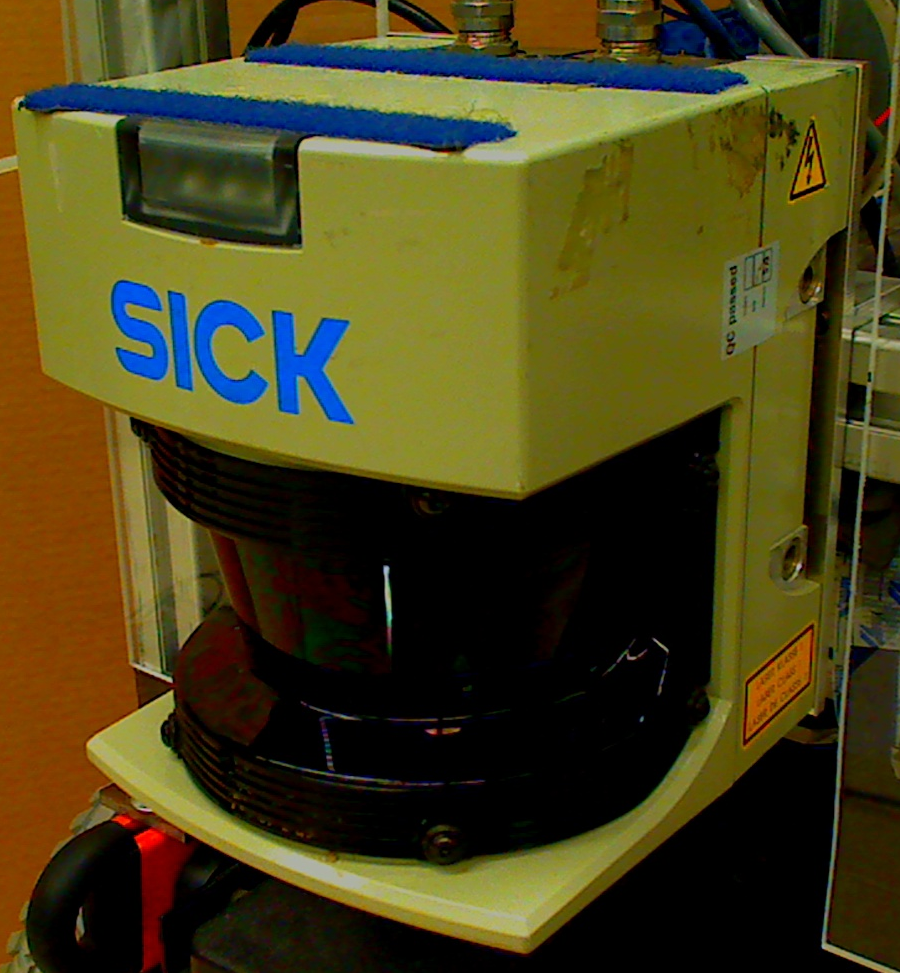
\includegraphics[width=0.4\textwidth]{images/sick_lms291}\label{fig:sick_lms291}}
\hfill
\subfloat[Sample LIDAR Scan \autocite{WikipediaSICKScan}. Top: Sensor in blue, laser beam in red, environment in green. Bottom: Sample data points for a partially complete scan of the environment shown above (beam moves couterclockwise).]{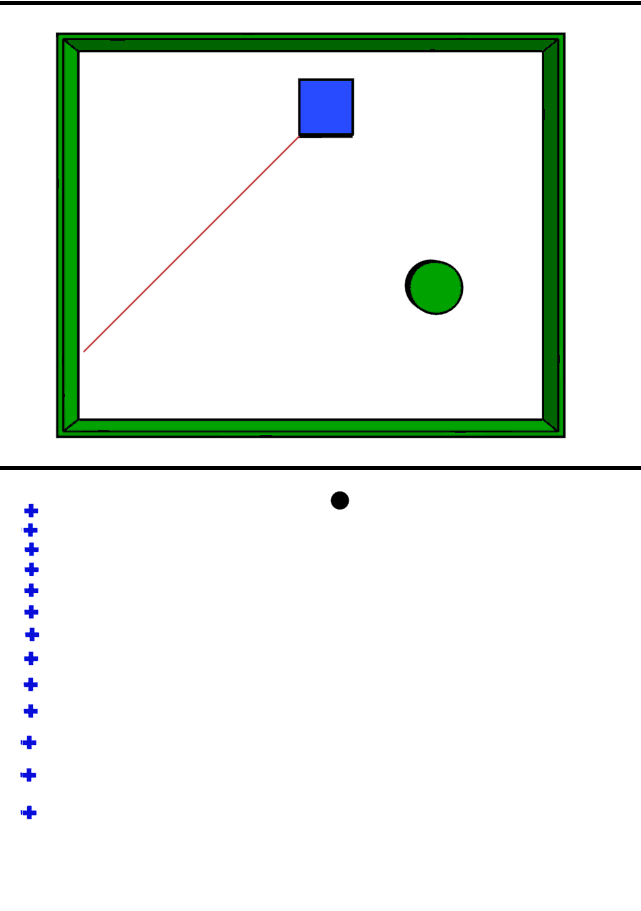
\includegraphics[width=0.4\textwidth]{images/sample_scan}\label{fig:sample_sick_scan}}
\caption{SICK LIDAR \& Sample LIDAR Scan}
\label{fig:sick_and_sample_scan}
\end{figure}

Harlie includes a number of other sensors, including cameras, a GPS receiver and sonar. Some like the GPS receiver, which allows for precise localization outdoors, would allow the methods described in the remainder of this thesis to function outdoors as well as indoors. Others such as the camera could augment the LIDAR for indoor localization \autocite{Harper2009}. Still others such as the sonar could be augmented and used to assist in detecting obstacles that the LIDAR cannot sense such as glass walls or materials with low infrared reflectivity.

\begin{figure}
\centering
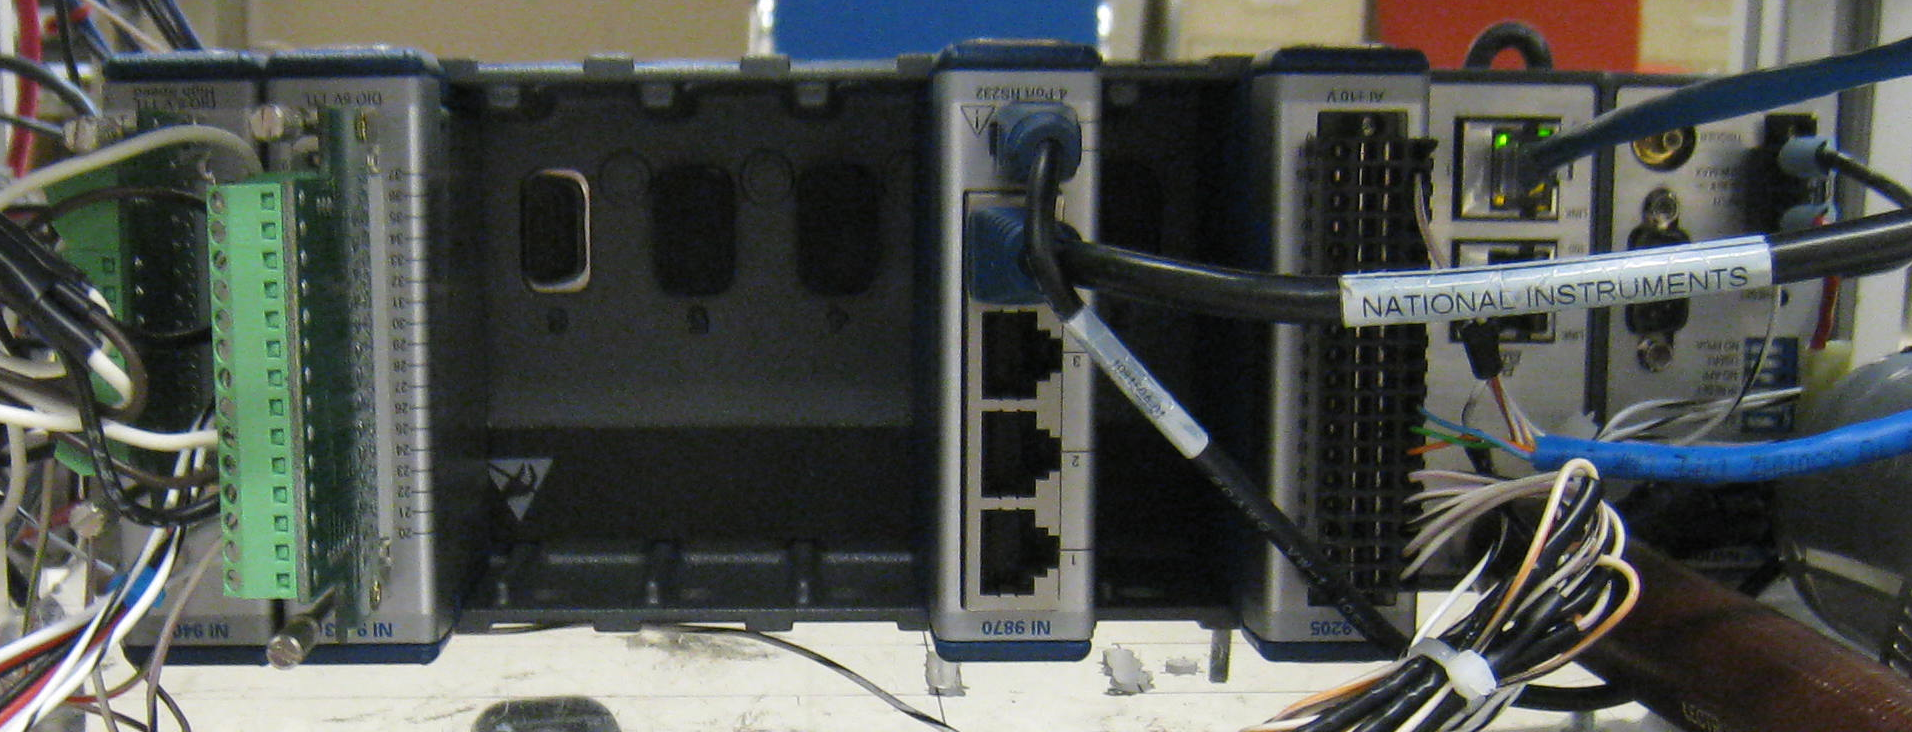
\includegraphics[width=0.75\textwidth]{images/cRIO}
\caption{NI cRIO with 4 IO modules installed and connected to onboard sensors \label{fig:crio}}
\end{figure}

HARLIE also includes a pair of computers. The first of these is a National Instruments CompactRIO (cRIO) that consists of a 400MHz PowerPC running VxWorks (a hard real-time operating system), a Xilinx FPGA and a large number of input/output modules for connecting to the different sensors \autocite{NIcRIO9074} (see \autoref{fig:crio}). HARLIE's cRIO is used for two main functions: relative localization (see \autoref{sec:localization} for details) and providing velocity control of the two drive wheels. The cRIO takes a translational (forward/backward) velocity as well as rotational velocity and converts them into a velocity for each drive wheel (see \autoref{subsubsec:harlie_ekf_encoder_measurement} for the equations used in this conversion). These individual wheel velocities are then used as the setpoint for the PID controller \todo{add ref to PID controller or something}for each wheel --- by using the wheel encoders for feedback to these PID algorithms, velocity commands are executed promptly and accurately even on different types of surfaces. Accurate velocity control offloads some work that would otherwise have to be done in the higher-level motion planning subsystems to ensure that the robot base is executing commands properly. The cRIO receives velocity commands and sends localization and status information to HARLIE's main computer via UDP over an Ethernet network.

The second computer on HARLIE is a custom-built Linux computer that includes an Intel Core i7 CPU clocked at 2.66GHz with up to eight simultaneous threads of execution and six gigabytes of RAM. This computer runs all of the obstacle mapping, absolute localization and motion planning discussed in later chapters. Since this computer is a standard Linux computer, many open-source libraries, programming languages and tools are available for use in those subsystems.

\subsection{Simulation}\label{subsec:simulation_setup}

While a physical platform is required for real world testing of a full navigation stack, field testing is impratical for gathering the amount of data requried to make any sort of generalization about the performance characteristics of the algorithms involved. In order to gather such a large amount of data pratically, a simulated robot was setup to mimic the characteristics of HARLIE. To do this, a number of steps were carried out.

\begin{figure}
\centering
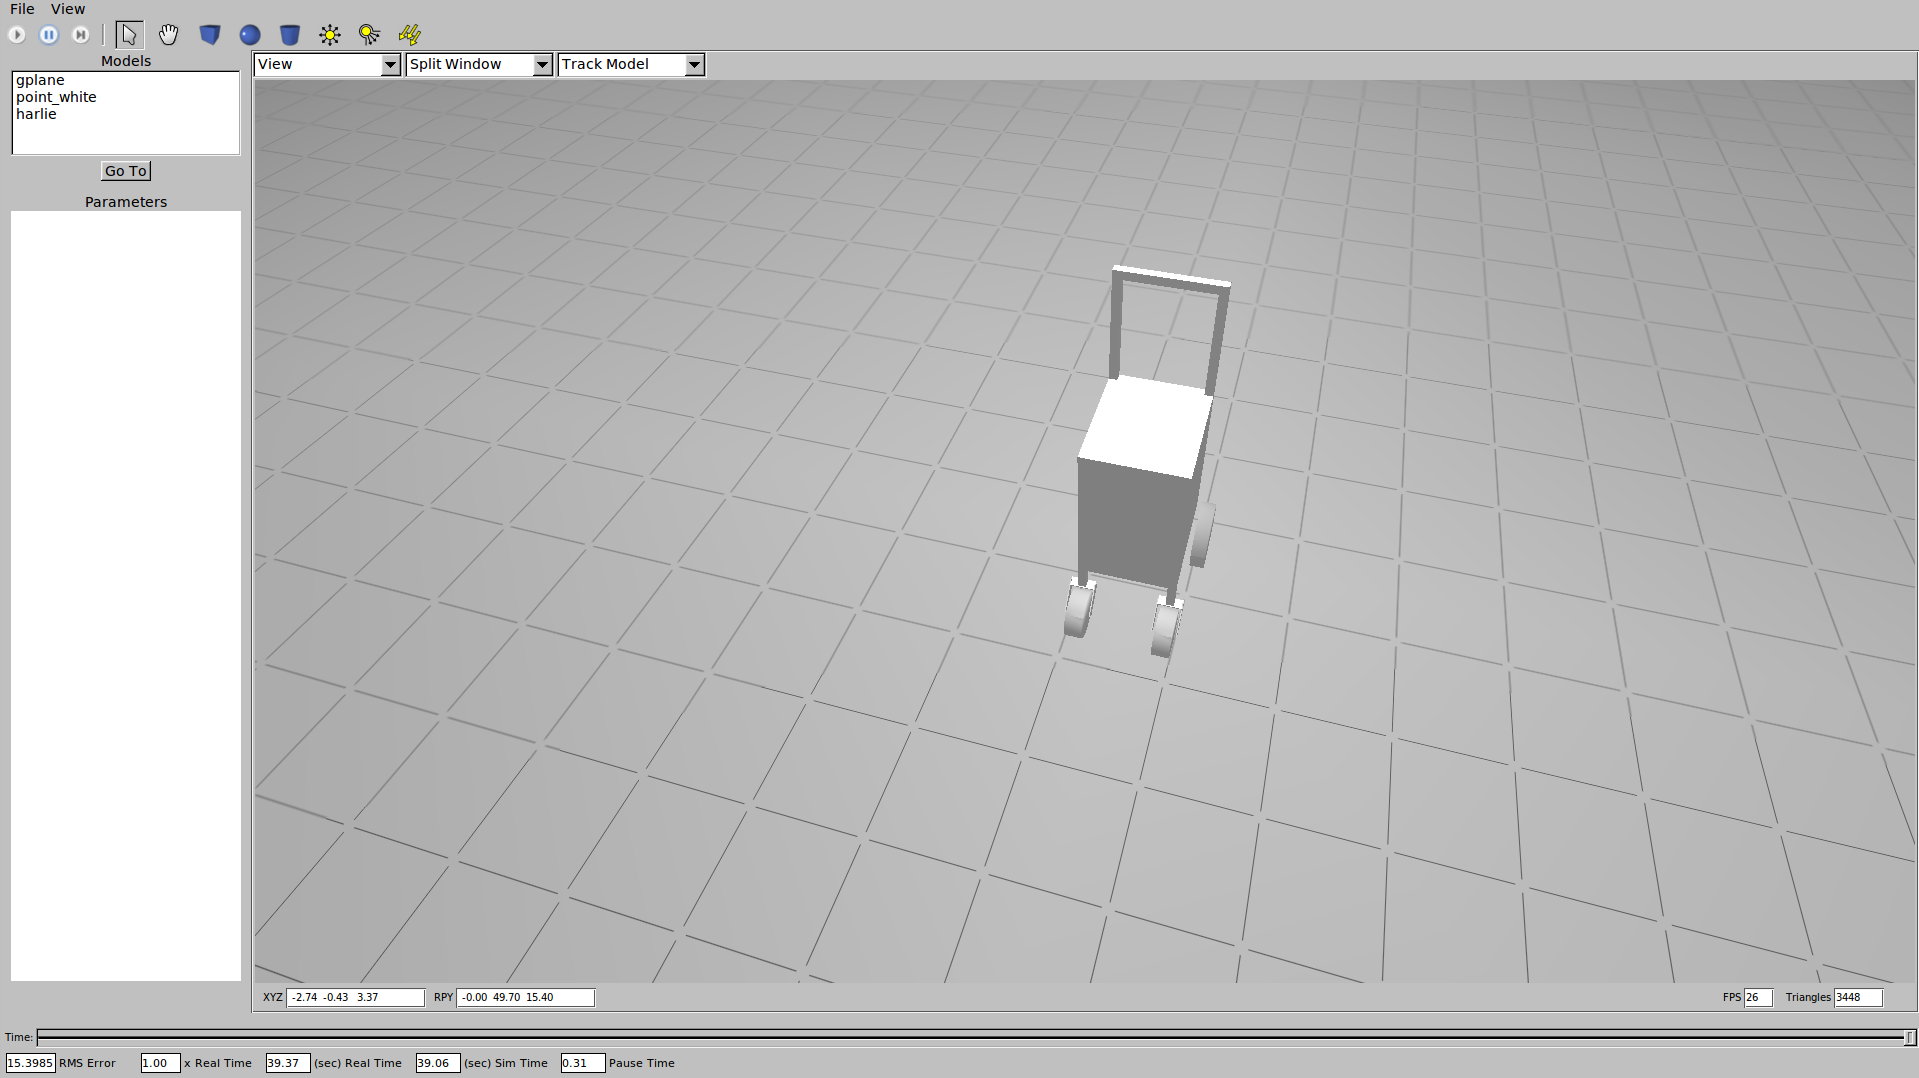
\includegraphics[width=0.80\textwidth]{images/harlie_in_gazebo}
\caption{HARLIE in the Gazebo Simulator \label{fig:harlie_in_gazebo}}
\end{figure}

First, a reasonably accurate model of HARLIE's physical structure and characteristics was created. This includes things such as the locations of the wheels and LIDAR, HARLIE's mass and estimates of the inertial constants of the wheels and the configuration and noise model for HARLIE's LIDAR (see \autoref{fig:harlie_in_gazebo}). Next, all of this information was fed into the Gazebo simulator \autocite{Koenig04designand}, which then uses those characteristics to do a 3D full-physics simulation of HARLIE. This setup was used to validate changes to the algorithms before testing on HARLIE as well as for gathering the data used to analyze the steering algortihms' attraction regions.

